\documentclass[skript.tex]{subfiles}

\begin{document}
	\begin{defin}[Faltung]
		Für integrierbare $f,g \colon \mbb{R}^n\to\mbb{R}$ setzen wir:
		\[
			(f\ast g)(x) = \int_{\mbb{R}^n} f(x-y)g(y) \md\lambda^n(y)
			= \int_{\mbb{R}^n} f(y)g(x-y) \md\lambda^n(y)
		\] und bezeichnen den Ausdruck $f \ast g$ als \emph{Faltung}.
	\end{defin}
	Die Faltung ist selbst integrierbar, wir haben nämlich:
	\begin{align*}
		\int_{\mbb{R}^n}\abs{f \ast g} \md \lambda^n
		&\leq \int_{\mbb{R}^n} \int_{\mbb{R}^n} \abs{f(x-y)}\abs{g(y)} \md \lambda^n(y)  \md \lambda^n(x) \\
		&\darrow{\text{Fubini}}{=} \int_{\mbb{R}^n} \underbrace{\int_{\mbb{R}^n} \abs{f(x-y)} \md \lambda^n(x)}_{\mathclap{
			\uarrow{\text{Trafo.}}{=} \int_{\mbb{R}^n} \abs{f(x)} \md \lambda^n(x) = \norm{f}_{L^1}
		}} \abs{g(y)} \md \lambda^n(y) = \norm{f}_{L^1} \norm{g}_{L^1} < \infty
	\end{align*}
	
	\begin{lem}
		Die Faltung besitzt die folgenden Eigenschaften:
		\begin{enumerate}[(i)]
			\item Für $x \in \mbb{R}^n$ ist die Funktion $f(x-\bcdot)g(\bcdot)$ genau dann integrierbar, wenn $f(\bcdot)g(x-\bcdot)$ integrierbar ist und in diesem Fall gilt
			\[
				(f \ast g)(x) = (g \ast f)(x).
			\]
			
			\item Für $\phi \in C_c^k(\mbb{R}^n),\, k\in\N$ und $f \in L_\text{loc}^1(\mbb{R}^n)$ folgt $f \ast \phi \in C^k(\mbb{R}^n)$ und
			\[
				\del_\alpha(f\ast\phi) = (\del_\alpha\phi)\ast f
			\]
			für jede partielle Ableitung einer Ordnung $\leq k$. Dabei ist $\alpha$ ein sogenannter \emph{Multiindex}.
			
			\item Für $\phi \in C_c^k(\mbb{R}^n),\, k\in\N,\, f \in L_c^1(\mbb{R}^n)$ (d.\,h. es gibt einen Räpresentanten mit kompaktem Träger) ist
			\[
				f\ast\phi \in C_c^k(\mbb{R}^n)
			\]
			
			\item Für $\phi \in L^1(\mbb{R}^n),\, f \in L^p(\mbb{R}^n),\, p \in [1,\infty]$ gilt auch $f \ast \phi \in L^p(\mbb{R}^n)$ und wir haben
			\[
				\norm{f\ast\phi}_{L^p} \leq \norm{\phi}_{L^1} \norm{f}_{L^p}.\quad\text{(Young-Ungleichung)}
			\]
		\end{enumerate}
	\end{lem}
	\begin{proof}
		\hfill
		\begin{enumerate}[(i)]
			\item folgt durch Koordinatenwechsel (vgl. Bemerkung vor Trafo-Satz).
			
			\item folgt induktiv durch vertauschen von Differentiation und Integration (siehe Übungsaufgabe 9).
			
			\item Ist $\supp f \cup \supp \phi \sbs B_R(0)$ für $R > 0$, so erhalten wir für $x \in \mbb{R}^n$
			\begin{align*}
				(f \ast \phi)(x) &\overset{\text{Def.}}{=} \int_{\mbb{R}^n} f(y)\phi(x-y)\md\lambda^n(y) \overset{\boldsymbol !}{\neq} 0 \\
				&\implies y,x-y \overset{\boldsymbol !}{\in} B_R(0) \implies x = (x-y)+y \overset{\boldsymbol !}{\in} B_{2R}(0).
			\end{align*}
			Demnach ist $\supp f\ast\phi \in B_{2R}(0)$.
			
			\item Für $p=\infty$ ist
			\begin{align*}
				\norm{f\ast\phi}_{L^\infty} &= \norm{\int_{\mbb{R}^n} f(y) \phi(\bcdot-y) \md\lambda^n(y)}_{L^\infty} \\ &\darrow{\text{Hölder}}{\leq} \norm{f}_{L^\infty} \norm{\int_{\mbb{R}^n}\phi(\bcdot-y) \md\lambda^n(y)}_{L^\infty} = \norm{\phi}_{L^1}\norm{f}_{L^\infty}
			\end{align*}
			Sei nun $p \in [1,\infty)$. Wir können \OE\  $\norm{\phi}_{L^1} = 1$ annehmen.\\
			Anwendung der Jensenschen Ungleichung liefert (mit $\varphi(\xi) = \abs{\xi}^p$, $\md\mu=\abs{\phi}\md\lambda^n$, also $\mu$ ein Wahrscheinlichkeitsmaß)
			\begin{align*}
				\norm{f\ast\phi}_{L^p}^p &\leq \int_{\mbb{R}^n}\abs{\int_{\mbb{R}^n} \abs{f(x-y)} \abs{\phi(y)} \md\lambda^n(y)}^p \md \lambda^n(x)
				\\ 
				&= \int_{\mbb{R}^n} \underbrace{\varphi\left(\int_{\mbb{R}^n} \abs{f(x-y)} \md\mu(y)\right)}_{
					\mathclap{
						\leq \int_{\mbb{R}^n} 	\varphi(\abs{f(x-y)}) \md\mu(y)
					}
				} \md \lambda^n(x) \\
				&\uarrow{\text{Fubini}}{\leqq} \int_{\mbb{R}^n}\underbrace{\int_{\mbb{R}^n} \abs{f(x-y)}^p \md\lambda^n(x)}_{\uarrow{\text{Trafo.}}{=} \norm{f}_{L^p}^p} \md\mu(y) = \norm{f}_{L^p}^p
			\end{align*}
		\end{enumerate}
	\end{proof}
	
	\newpage
	\begin{defin}
		Eine Familie $(\phi_\epsilon)_{\epsilon>0}$ integrierbarer Funktionen $\mbb{R}^n \to \mbb{R}$ heißt \emph{approximative Identität}, falls\\
		\begin{enumerate}[(i)]
		\begin{minipage}[b]{0.5\textwidth}
			\item $\sup_{\epsilon>0} \norm{\phi_\epsilon}_L^1 < \infty$\\(auch häufig zu finden: $\phi_\epsilon \geq 0 \quad\forall\epsilon > 0$)
			\item $\displaystyle{\int_{\mbb{R}^n}\phi_\epsilon\md\lambda^n = 1\quad\forall \epsilon > 0}$
			\item $\displaystyle{\int_{\mbb{R}^n\setminus B_r(0)} \abs{\phi_\epsilon} \md\lambda^n \xrightarrow{\epsilon\searrow 0}0 \quad\forall r>0}$
		\end{minipage}
		\begin{minipage}{0.3\textwidth}
			\begin{tikzpicture}[scale=1.2]
			\draw[draw=none,fill=green,fill opacity=.3] plot[smooth, tension=1] coordinates{(0,0)(1,.2)(2.5,1)(4,.2)(5,0)};
			\draw[draw=none,fill=yellow,fill opacity=.5] plot[smooth, tension=.5] coordinates{(0,0)(1.8,.3)(2.2,1.7)(2.5,2)(2.8,1.7)(3.2,.3)(5,0)};
			\draw[draw=none,fill=red,fill opacity=.3] plot[smooth, tension=.5] coordinates{(0,0)(2.05,.3)(2.4,2.7)(2.5,3)(2.6,2.7)(2.95,.3)(5,0)};
			
			\draw[fill=white,draw=white] (2.1,0) rectangle (2.9,3.5);
			
			\definecolor{darkgreen}{rgb}{0,.5,0}
			\definecolor{darkyellow}{rgb}{.7,.7,0}
			\draw[draw=darkgreen] plot[smooth, tension=1] coordinates{(0,0)(1,.2)(2.5,1)(4,.2)(5,0)};
			\draw[draw=darkyellow] plot[smooth, tension=.5] coordinates{(0,0)(1.8,.3)(2.2,1.7)(2.5,2)(2.8,1.7)(3.2,.3)(5,0)};
			\draw[draw=red] plot[smooth, tension=.5] coordinates{(0,0)(2.05,.3)(2.4,2.7)(2.5,3)(2.6,2.7)(2.95,.3)(5,0)};
			
			\node[color=darkgreen] at (3.9,0.6) {$\phi_1$};
			\node[color=darkyellow] at (3.3,1.5) {$\phi_{\nicefrac{1}{2}}$};
			\node[color=red] at (3,2.4) {$\phi_{\nicefrac{1}{3}}$};
			
			\draw[->,ultra thick] (0,0)--(5,0);
			\draw[->,ultra thick] (2.5,0-.5)--(2.5,3.5);
			\draw[thick,decoration={brace,mirror},decorate] (2.55,-.1)--node[below=1mm]{$r$}(2.9,-.1);
			\end{tikzpicture}
		\end{minipage}
		\end{enumerate}
	Ein \emph{Glättungskern} (engl. \emph{mollifier}) ist eine nicht-negative Funktion $\phi \in C_c^0(\mbb{R}^n)$ mit $\norm{\phi}_{L^1}=1$.
	\end{defin}

	\begin{bem}
		Aus jedem Glättungskern $\phi$ erhält man vermöge
		\[
			\phi_\epsilon(x) = \epsilon^{-n}\phi\left(\frac{x}{\epsilon}\right),\quad\phi\in C_c^\infty(\mbb{R}^n)
		\]
		eine approximative Identität. Häufig zum Einsatz kommt der Standard-Glättungskern
		\[
			x \mapsto
			\begin{cases}
				\exp\left(\frac{1}{\abs{x}^2-1}\right), &\text{falls } \abs{x} < 1 \\
				0, &\text{falls } \abs{x} \geq 1
			\end{cases}
			\quad\text{(Übungsaufgabe 25)}.
		\]
	\end{bem}
	
	Für den Rest dieses Kapitels verwenden wir (ohne Beweis) die Regularität des Lebesgue-Maßes.
	
	\begin{lem}
		Sei $(\phi_\epsilon)_{\epsilon>0}$ eine approximative Identität und $f \in L^p(\mbb{R}^n),\ p\in[1,\infty)$.\\
		Dann gilt
		\[
			\norm{f \ast \phi_\epsilon-f}_{L^p} \xrightarrow{\epsilon\searrow 0} 0.
		\]
	\end{lem}
	\begin{proof}
		Sei zunächst $f \in C_c^0(\mbb{R}^n)$. Wir fixieren ein $\delta>0$ und erhalten aufgrund der gleichmäßigen Stetigkeit (nach dem Satz von Heine) von $f$
		\[
			\abs{f(x-y)-f(x)} \xrightarrow{\abs{y}\searrow0} 0\quad\text{\emph{gleichmäßig} in } x.
		\]
		Weiterhin erhalten wir aufgrund des kompakten Trägers für $\abs{y} < r$ ($r$ hinreichend klein)
		\begin{align*}
			\norm{f(\bcdot-y)-f)}_{L^p} &\overset{\footnotemark}{=}
			 \left(\int_{B_r(\supp f)}\abs{f(x-y)-f(x)}^p \md\lambda^n(x)\right)^{\nicefrac{1}{p}}\\
			&\leq \norm{f(\bcdot-y)-f}_{L^\infty}\left(\int_{B_r(\supp f)}1^p\md\lambda^n(x)\right)^{\nicefrac{1}{p}}\\
			&\leq \frac{\delta}{2\sup_{\epsilon>0}\norm{\phi_\epsilon}_{L^1}}\quad\text{für $r$ hinreichend klein.}
		\end{align*}
		\footnotetext{Für $E \sbs \mbb{R}^n$ definiere $B_s(E) \coloneqq \bigcup_{\xi\in E} B_s(\xi)$.}
		\newpage
		Nun ist weiter
		\[
			(f\ast\phi_\epsilon)(x)-f(x) = \int_{\mbb{R}^n} \phi_\epsilon(y)(f(x-y)-f(x)) \md\lambda^n(y)
		\]
		und die Minkowski-Ungleichung (\emph{Satz 9}) liefert
		\[
			\norm{(f\ast\phi_\epsilon)-f}_{L^p} \darrow{\text{$\Delta$-Ungl.}}{\leq} \underbrace{
				\norm{\int_{B_r(0)} \phi_\epsilon(y)(f(\bcdot-y)-f(\bcdot)) \md\lambda^n(y)}_{L^p}
			}_{(\ast)}+\underbrace{
			\norm{\int_{\mbb{R}^n \setminus B_r(0)} \phi_\epsilon(y)(f(\bcdot-y)-f(\bcdot)) \md\lambda^n(y)}_{L^p}
			}_{(\ast\ast)},
		\]
		wobei man die beiden Terme weiter abschätzen kann:
		\begin{align*}
			(\ast) &\leq \int_{B_r(0)}\abs{\phi_\epsilon(y)}\underbrace{\norm{f(\bcdot-y)-f)}_{L^p}}_{\leq \delta/(2\sup_{\epsilon>0}\norm{\phi_\epsilon}_{L^1})} \md\lambda^n(y) \leq \delta/2 \\
			(\ast\ast) &\leq \int_{\mbb{R}^n\setminus B_r(0)}\abs{\phi_\epsilon(y)}\underbrace{\norm{f(\bcdot-y)-f)}_{L^p}}_{\leq 2\norm{f}_{L^p}} \md\lambda^n(y) \leq 2\norm{f}_{L^p} \int_{\mbb{R}^n\setminus B_r(0)}\abs{\phi_\epsilon(y)} \md\lambda^n(y)
		\end{align*}
		$(\ast\ast)\leq\frac{\delta}{2}$ für hinreichend kleine $\epsilon>0$.\\
		Somit ist die Behauptung für $f \in C_c^0(\mbb{R}^n)$ gezeigt.\\
		Da diese Funktionen nach \emph{Satz 15} dicht in $L^p(\mbb{R}^n)$ liegen, wählen wir für eine allgemeine Funktion $f \in L^p(\mbb{R}^n)$ eine Folge $(f_k)_{k\in\N} \sbs C_c^0(\mbb{R}^n)$ mit $\norm{f_k-f}_{L^p} \xrightarrow{k\to\infty} 0$ und erhalten
		\begin{align*}
			\norm{f\ast\phi_\epsilon-f}_{L^p} &\leq \underbrace{\norm{f\ast\phi_\epsilon-f_k\ast\phi_\epsilon}_{L^p}}_{=\norm{(f-f_k)\ast\phi_\epsilon}_{L^p}}
			+\underbrace{\norm{f_k\ast\phi_\epsilon-f_k}_{L^p}}_{\substack{\xrightarrow{\epsilon\searrow 0} 0\\\text{ f. festes $k$}}}
			+\underbrace{\norm{f_k-f}_{L^p}}_{\xrightarrow{k\to\infty} 0}\\
			&\leq \underbrace{\norm{f-f_k}_{L^p}}_{\xrightarrow{k\to\infty} 0}
			\underbrace{\norm{\phi_\epsilon}_{L^1}}_{\leq M}
		\end{align*}
		Wähle erst $k$ hinreichend groß und dann $\epsilon$ hinreichend klein $\implies$ Behauptung.
	\end{proof}

	\begin{theorem}
		Sei $\Omega\sbs\mbb{R}^n$ offen. Dann liegt die Menge $C_c^\infty(\Omega)$ aller glatten Funktionen mit kompaktem Träger dicht in $L^p(\Omega)$ für $p\in[1,\infty)$.
	\end{theorem}
	\begin{proof}
		Nach \emph{Satz 15} genügt es zu zeigen, dass jede Funktion aus $C_c^0(\mbb{R}^n)$ durch Funktionen aus $C_c^\infty(\mbb{R}^n)$ approximiert werden kann, denn wir können $f\vert_{\mbb{R}^n\setminus\Omega} = 0$ setzen.\\
		Wir wählen einen Glättungskern $\phi$ und schließen, dass $f\ast\phi_\epsilon$ kompakte Träger hat und $C^\infty$-glatt ist (vgl. \emph{Lemma 17(iii)}).\\
		Die Behauptung folgt nun aus \emph{Lemma 20}.
	\end{proof}
	
\end{document}